This section describes the purpose, use and intended user audience for the Beverage Management app. Beverage Management app is an android application that provides an efficient way to manage large collection of beverages using smartphone.

\subsection{Purpose and Use}
Beverage Management is an android application that works as a virtual inventory and allows user to effectively manage and keep track of several beverages. Users can use this app to keep track of name, storage location, brewery, style, volume, manufactured date and best before date. It also allows user to search and sort the beverages according to the date, style etc.

\subsection{Intended Audience}
The intended audience for this application are those people who have large collection of beverages in their home and are looking for easy ways to manage them free of cost. It can also be used in local grocery stores, bars and restaurants to keep track of their beverage inventory. Our app is intended for general use but it can certainly be expanded into a more complex inventory management system with additional features.  

\begin{figure}[h!]
	\centering
   	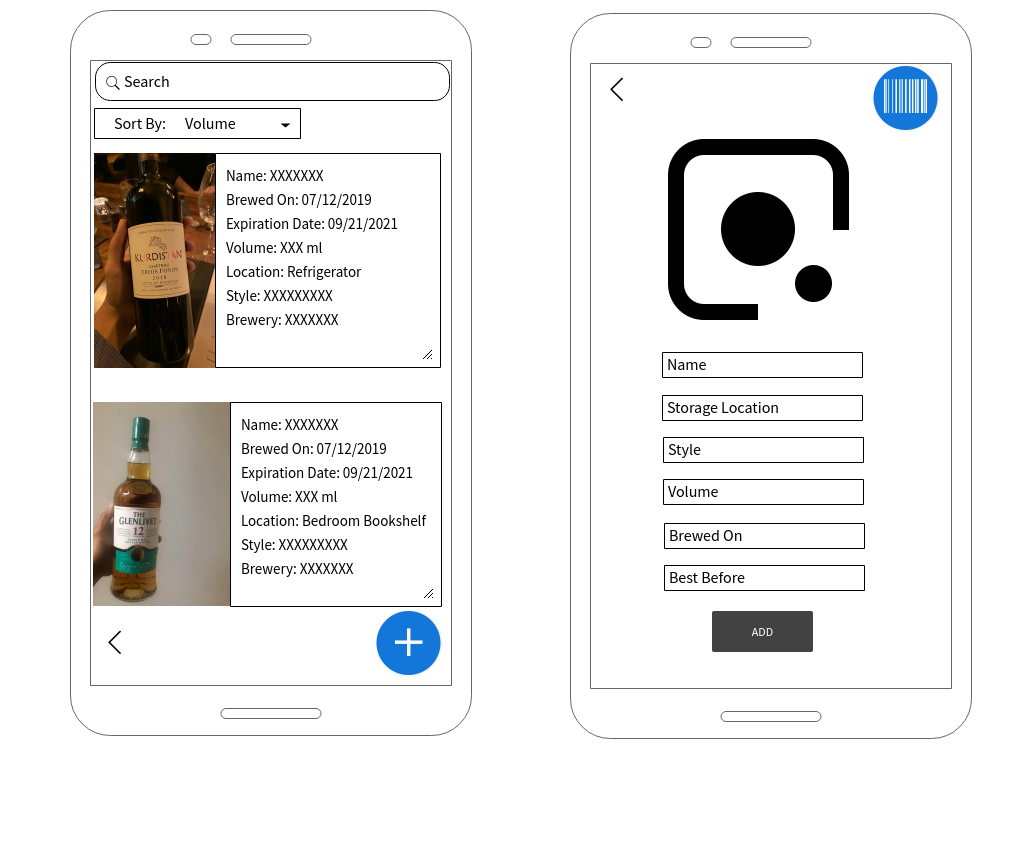
\includegraphics[width=0.60\textwidth]{images/CD.png}
    \caption{ conceptual drawing of Beverage Management App (Home screen and Add screen) }
\end{figure}
